%!Mode:: "TeX:UTF-8"
\documentclass[a4paper,11pt,UTF8]{ctexart}

\usepackage{indentfirst} %缩进
\usepackage{xeCJK}    %使用系统字体
\usepackage{bm}       %粗体
\usepackage{fancyhdr} %自定义页眉页脚
\pagestyle{plain}                   %不设置页眉页脚
\usepackage{amsmath, amsthm, amssymb, amsfonts} %数学公式
\usepackage[a4paper,left=3cm,right=3cm,top=3.5cm,bottom=3.5cm]{geometry}
\usepackage{booktabs} %插入表格
\usepackage[section]{placeins} %避免浮动
\usepackage{listings} %插入代码
\usepackage{ctex}     %中文宏包
\usepackage[svgnames, table]{xcolor} %彩色表格
\usepackage{algorithm}          %伪代码
\usepackage{algorithmicx}
\usepackage{algpseudocode}
\usepackage{algorithm,algpseudocode,float}
\usepackage{lipsum}
\usepackage{enumitem}           %调整列举环境
\usepackage{url}
\usepackage{fontspec,xunicode}
\usepackage{subfigure}
\defaultfontfeatures{Mapping=tex-text} %如果没有它,会有一些 tex 特殊字符无法正常使用,比如连字符。

\usepackage{graphicx}
\graphicspath{{imgs/}}

%%%%%%%%%%%%%%%%%%%%%%%%%%%%%%%%%%%%%%%%%%%%%%%%%%%%%%%%%%%%%%%%
% 缩进及行间距
%%%%%%%%%%%%%%%%%%%%%%%%%%%%%%%%%%%%%%%%%%%%%%%%%%%%%%%%%%%%%%%%
\setlength{\parindent}{22bp} %重新定义缩进长度
\linespread{1}

%%%%%%%%%%%%%%%%%%%%%%%%%%%%%%%%%%%%%%%%%%%%%%%%%%%%%%%%%%%%%%%%
% 图的标题行间距设置
%%%%%%%%%%%%%%%%%%%%%%%%%%%%%%%%%%%%%%%%%%%%%%%%%%%%%%%%%%%%%%%%
\newcommand{\bottomcaption}{%
\setlength{\abovecaptionskip}{6bp}%
\setlength{\belowcaptionskip}{6bp}%
\caption}


%%%%%%%%%%%%%%%%%%%%%%%%%%%%%%%%%%%%%%%%%%%%%%%%%%%%%%%%%%%%%%%%
% 字体定义
%%%%%%%%%%%%%%%%%%%%%%%%%%%%%%%%%%%%%%%%%%%%%%%%%%%%%%%%%%%%%%%%
\setmainfont{Times New Roman}  %默认英文字体.serif是有衬线字体sans serif无衬线字体
\setmonofont{Consolas}
\setCJKmainfont[ItalicFont={楷体}, BoldFont={黑体}]{宋体}%衬线字体 缺省中文字体为
\setCJKsansfont{黑体}
\punctstyle{hangmobanjiao}
%-----------------------xeCJK下设置中文字体------------------------------%
\setCJKfamilyfont{song}{SimSun}                             %宋体 song
\newcommand{\song}{\CJKfamily{song}}
\setCJKfamilyfont{fs}{FangSong}                      %仿宋  fs
\newcommand{\fs}{\CJKfamily{fs}} 
\let\kaishu\relax                                    %重定义楷体,打开假粗体
\newCJKfontfamily\kaishu{KaiTi}[AutoFakeBold] 
%\setCJKfamilyfont{ktgb}{KaiTi_GB2312}                      %楷体 GB2312
%\newcommand{\ktgb}{\CJKfamily{ktgb}}
\setCJKfamilyfont{yh}{Microsoft YaHei}                    %微软雅黑 yh
\newcommand{\yh}{\CJKfamily{yh}}
\setCJKfamilyfont{hei}{SimHei}                              %黑体  hei
\newcommand{\hei}{\CJKfamily{hei}}
\setCJKfamilyfont{hwxk}{STXingkai}                                %华文行楷  hwxk
\newcommand{\hwxk}{\CJKfamily{hwxk}}
%------------------------------设置字体大小------------------------%
\newcommand{\chuhao}{\fontsize{42bp}{63bp}\selectfont}     %初号, 1.5倍行距
\newcommand{\xiaochuhao}{\fontsize{36bp}{36bp}\selectfont} %小初号,单倍行距
\newcommand{\yihao}{\fontsize{26bp}{39bp}\selectfont}        % 一号, 1.5 倍行距
\newcommand{\erhao}{\fontsize{22bp}{33bp}\selectfont}        % 二号, 1.5倍行距
\newcommand{\xiaoerhao}{\fontsize{18bp}{18bp}\selectfont}       % 小二, 单倍行距
\newcommand{\sanhao}{\fontsize{16bp}{24bp}\selectfont}       % 三号, 1.5倍行距
\newcommand{\xiaosanhao}{\fontsize{15bp}{22bp}\selectfont}      % 小三, 1.5倍行距
\newcommand{\sihao}{\fontsize{14bp}{21bp}\selectfont}        % 四号, 1.5 倍行距
\newcommand{\banxiaosi}{\fontsize{13bp}{20bp}\selectfont}  % 半小四, 20pt行距
\newcommand{\xiaosihao}{\fontsize{12bp}{20bp}\selectfont}       % 小四, 20pt行距
\newcommand{\dawuhao}{\fontsize{11bp}{11bp}\selectfont}      % 大五号, 单倍行距
\newcommand{\wuhao}{\fontsize{10.5bp}{10.5bp}\selectfont}   % 五号, 单倍行距
\newcommand{\xiaowuhao}{\fontsize{9bp}{9bp}\selectfont}   %小五号,单倍行距
%------------------------------重定义normalize------------------------%
\renewcommand{\normalsize}{\fontsize{12bp}{20bp}\selectfont}


%%%%%%%%%%%%%%%%%%%%%%%%%%%%%%%%%%%%%%%%%%%%%%%%%%%%%%%%%%%%%%%%
% 图题字体大小相同
%%%%%%%%%%%%%%%%%%%%%%%%%%%%%%%%%%%%%%%%%%%%%%%%%%%%%%%%%%%%%%%%
\usepackage{caption}
\captionsetup{font={footnotesize}}   % footnotesize = 9bp
\captionsetup[lstlisting]{font={footnotesize}}

%%%%%%%%%%%%%%%%%%%%%%%%%%%%%%%%%%%%%%%%%%%%%%%%%%%%%%%%%%%%%%%%
% 重定义枚举编号为 1),2)...
%%%%%%%%%%%%%%%%%%%%%%%%%%%%%%%%%%%%%%%%%%%%%%%%%%%%%%%%%%%%%%%%
\renewcommand{\labelenumi}{\theenumi)}


%%%%%%%%%%%%%%%%%%%%%%%%%%%%%%%%%%%%%%%%%%%%%%%%%%%%%%%%%%%%%%%%
% 重定义section标题
%%%%%%%%%%%%%%%%%%%%%%%%%%%%%%%%%%%%%%%%%%%%%%%%%%%%%%%%%%%%%%%%
\CTEXsetup[format={\CJKfamily{zhhei}\zihao{4}},number={\chinese{section}},name={,、~},aftername={},indent={0bp},beforeskip={6bp},afterskip={6bp},format+={\flushleft}]{section}
% \CTEXsetup[format={\Large\bfseries\CJKfamily{zhkai}\zihao{5}},name={(,)},number={\chinese{subsection}},aftername={},indent={22bp},beforeskip={6bp},afterskip={6bp}]{subsection}
\CTEXsetup[number={\chinese{section}},name={附录, ~~ }]{appendix}



%%%%%%%%%%%%%%%%%%%%%%%%%%%%%%%%%%%%%%%%%%%%%%%%%%%%%%%%%%%%%%%%
% 标题名称中文化
%%%%%%%%%%%%%%%%%%%%%%%%%%%%%%%%%%%%%%%%%%%%%%%%%%%%%%%%%%%%%%%%
\renewcommand\figurename{\hei 图}
\renewcommand\tablename{\hei 表}
\renewcommand\lstlistingname{\hei 代码}
\renewcommand{\algorithmicrequire}{\textbf{输入:}}
\renewcommand{\algorithmicensure}{\textbf{输出:}}
\newtheorem{define}{定义}


%%%%%%%%%%%%%%%%%%%%%%%%%%%%%%%%%%%%%%%%%%%%%%%%%%%%%%%%%%%%%%%%
% 列表设置
%%%%%%%%%%%%%%%%%%%%%%%%%%%%%%%%%%%%%%%%%%%%%%%%%%%%%%%%%%%%%%%%
\setlist[enumerate,1]{itemindent=22bp,listparindent=\parindent,itemsep=0mm,partopsep=.7mm,parsep=0ex,labelsep=1.5mm,topsep=0.7mm}
\setlist[enumerate,2]{label=\alph*),leftmargin=1.5em}  %二级item设置
%\setitemize{itemindent=38bp,leftmargin=0bp,itemsep=-0.4ex,listparindent=26bp,partopsep=0bp,parsep=0.5ex,topsep=-0.25ex}
%\setdescription{itemindent=38bp,leftmargin=0bp,itemsep=-0.4ex,listparindent=26bp,partopsep=0bp,parsep=0.5ex,topsep=-0.25ex}

%%%%%%%%%%%%%%%%%%%%%%%%%%%%%%%%%%%%%%%%%%%%%%%%%%%%%%%%%%%%%%%%
% 代码设置
%%%%%%%%%%%%%%%%%%%%%%%%%%%%%%%%%%%%%%%%%%%%%%%%%%%%%%%%%%%%%%%%
\lstset{
 columns=fixed,
 numbers=left,                                        % 在左侧显示行号
 numberstyle=\tiny\color{gray},                       % 设定行号格式
 frame=single,                                        % 单线背景边框
 breaklines=true,                                     % 设定LaTeX对过长的代码行进行自动换行
 keywordstyle=\color[RGB]{40,40,255},                 % 设定关键字颜色
 numberstyle=\footnotesize\color{darkgray},
 commentstyle=\it\color[RGB]{0,96,96},                % 设置代码注释的格式
 stringstyle=\rmfamily\slshape\color[RGB]{128,0,0},   % 设置字符串格式
 showstringspaces=false,                              % 不显示字符串中的空格
 language=java,                                        % 设置语言
 basicstyle=\linespread{1.0}\xiaowuhao\ttfamily,                      % 字体字号
 %lineskip=10bp,
 %baselinestretch=1,
}

%%%%%%%%%%%%%%%%%%%%%%%%%%%%%%%%%%%%%%%%%%%%%%%%%%%%%%%%%%%%%%%%
% 伪代码分页
%%%%%%%%%%%%%%%%%%%%%%%%%%%%%%%%%%%%%%%%%%%%%%%%%%%%%%%%%%%%%%%%
\makeatletter
\renewcommand{\ALG@name}{算法}
\newenvironment{breakablealgorithm}
  {% \begin{breakablealgorithm}
   \begin{center}
     \refstepcounter{algorithm}% New algorithm
     \hrule height.8bp depth0bp \kern2bp% \@fs@pre for \@fs@ruled
     \renewcommand{\caption}[2][\relax]{% Make a new \caption
       {\raggedright\textbf{\ALG@name~\thealgorithm} ##2\par}%
       \ifx\relax##1\relax % #1 is \relax
         \addcontentsline{loa}{algorithm}{\protect\numberline{\thealgorithm}##2}%
       \else % #1 is not \relax
         \addcontentsline{loa}{algorithm}{\protect\numberline{\thealgorithm}##1}%
       \fi
       \kern2bp\hrule\kern2bp
     }
  }{% \end{breakablealgorithm}
     \kern2bp\hrule\relax% \@fs@post for \@fs@ruled
   \end{center}
  }
\makeatother



\begin{document}
\xiaosihao\song

\begin{titlepage}
\center{\yihao{\hwxk{电子科技大学\underline{计算机科学与工程}学院}}}
\vspace{6cm}
\center{\xiaochuhao{\kaishu{\bfseries 实~验~报~告}}}
\vspace{4cm}

\begin{center}
\begin{large}
\begin{tabular}{rc}
\xiaoerhao{\hei{学\qquad 号}}& \hspace{1.7cm}\xiaoerhao{\hei{2020080903009\hspace{1.7cm}}} \\
\cline{2-2}\\
\xiaoerhao{\hei{姓\qquad 名}}& \xiaoerhao{\hei{李皓}}\\
\cline{2-2}\\
\xiaoerhao{\hei{(实验)课程名称}}& \xiaoerhao{\hei{实验二~基元检测}}\\
\cline{2-2}\\
\xiaoerhao{\hei{教师}}& \xiaoerhao{\hei{任亚洲}}\\
\cline{2-2}\\

\end{tabular}
\end{large}
\end{center}
\vfill \hfill
\end{titlepage}
\clearpage

\centerline{\\[10bp]\erhao{\fs{电 ~子 ~科~ 技~ 大~ 学}}}

\centerline{\\[20bp]\yihao{\fs{实  ~~~~ 验  ~~~~ 报  ~~~~ 告}}}

\leftline{\\[10bp]\sihao{\hei{\hspace{1.5em} 学生姓名:李皓 \hfill 学号:2020080903009 \hfill 指导教师:任亚洲 }}}

% \leftline{\\[10bp]\sihao{\hei{\hspace{1.5em} 实验地点:信软楼西XXX \hfill }}}

% \leftline{\\[10bp]\sihao{\hei{\hspace{1.5em} 实验时间:第X周周X(X-X节) \hfill }}}

\setlength{\parskip}{0bp}  %定义段间距

\section{实验名称: 图像预处理}
% \section{实验学时: ~4}
\section{实验目的:}

熟练掌握基元检测的各种方法,包括边缘检测,以及角点检测。

\section{实验原理:}

\subsection{边缘检测}
像素值灰度的变化可以通过计算导数的方法来检测,我们一般使用一阶或者二阶导数进行检测。由于边缘的本质式灰度值的变化,边缘处的导数会有不同的相应情况。对于阶梯状边缘而言,一阶导数以在此处以阶跃形式出现,而其余地方数值为0;对于屋顶状边缘,一阶导数会出现上升沿和下降沿,此时二阶导数的极小值点处便是图像的边缘所在。

Sobel边缘导数算子常常分为两个方向,要获得边缘响应,我们需要根据两个偏导分量计算梯度矢量的模长。计算模长常常选择1范数、2范数、以及无穷范数。

\begin {figure}[h]
\centering % 居中显示
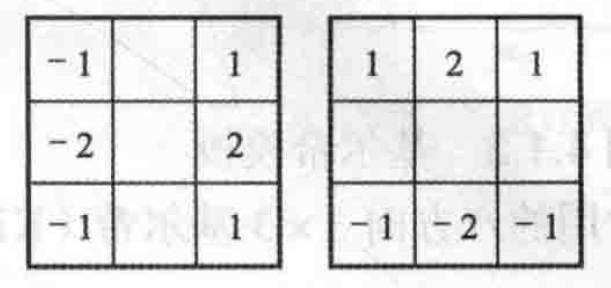
\includegraphics[width=0.5\textwidth]{sobel.png}
\caption{Sobel 算子} % 标题
\label{five}
\end {figure}

\subsection{角点检测}
我们以SUSAN算子介绍角点检测的方法。SUSAN算子只使用一个圆形模板来得到各向同性的响应。它不仅可以检测出图像中目标的边缘点,而且能较鲁棒地检测出图像中目标上的角点。

SUSAN算子将模板中各个像素的灰度都与模板中心的核像素的灰度进行比较,总有一部分模板区域像素的灰度与核像素的灰度相同或相似。这部分区域可称为核同值区(USAN区),即与核有相同值的区域。USAN区包含了很多与图像结构有关的信息。利用这种区域的尺寸、重心等统计量可以帮助检测图像中的边缘和角点。

利用上述USAN面积的变化可检测边缘或角点。具体说来,USAN面积较大(超过一半)时表明核像素处在图像中的灰度一致区域,在模板核接近边缘时该面积减少,而在接近角点时减少得更多,即USAN面积在角点处取得最小值。

\subsection{调研:高斯差分角点检测}

张小洪等人提出的\cite{1}高斯差分角点检测方法利用了不同$\sigma$值下的高斯卷积之差进行角点检测。如图(\ref{sigma})所示,利用一组卷积模板处理图像,观察可知角点在不同$\sigma$值下的变化程度不同,可以根据这一特性进行角点检测。
\begin {figure}[h]
\centering % 居中显示
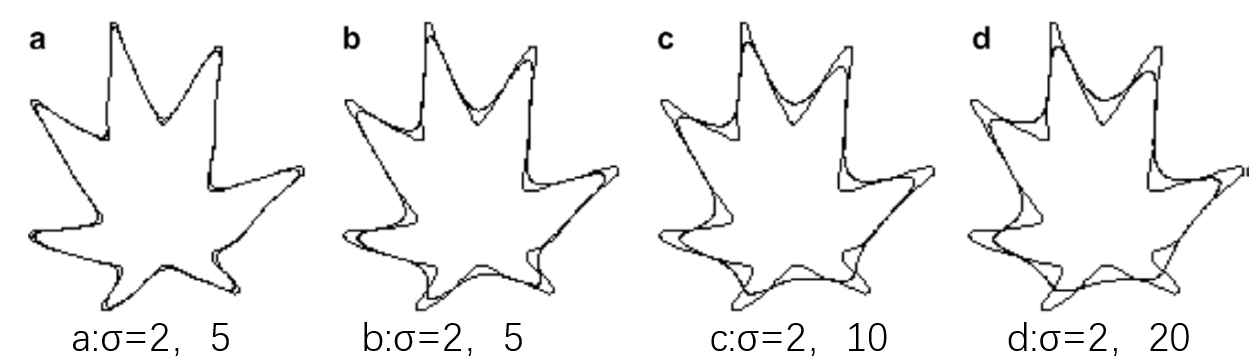
\includegraphics[width=\textwidth]{sigma.png}
\caption{不同$\sigma$值下角点检测的结果} % 标题
\label{sigma}
\end {figure}

我们定义高斯模板如下:
\begin{equation}
  G(u,\sigma) = \frac{1}{\sqrt{2\pi \sigma^2}}exp(-u^2/2\sigma^2)
\end{equation}

则卷积后的图像为:
\begin{equation}
  C(u,\sigma) =G(u,\sigma)*C(u) = (X(u,\sigma),Y(u,\sigma))
\end{equation}

计算不同$\sigma$数值下的差分图像$D$:
\begin{align}
  D(u,\sigma) =& C(u,m\sigma)-C(u,\sigma)\\
  [DoG*x(u)]^2+[DoG*y(u)]^2
\end{align}

其中$DoG$为高斯差分算子,计算如下:
\begin{equation}
  DoG = G(u,m\sigma) - G(u,\sigma)
\end{equation}

\section{实验内容:}
\begin{enumerate}
  \item 边缘检测:利用一阶导数算子(节4.1.2)进行边缘检测,可采用图4.1.2提供模板中的任意一个。在真实图像上测试,对一副真实图像,需画出图4.1.3的六副图像。
  \item 角点检测:利用SUSAN算子进行角点检测,并在真实图像上测试,将角点标识(参照图4.2.5)。
  \item 高斯差分角点检测:实现高斯差分角点检测,并且与SUSAN算子角点检测进行对比。
\end{enumerate}

\section{实验设备:}
\begin{itemize}
  \item Ubuntu 个人版 20.04 LTS
  \item Pycharm 2022.1
  \item Python 3.9
  \item PIL numpy matploit 等python库
\end{itemize}

\section{实验步骤:}
\subsection{使用Sobel算子进行图像边缘检测}
该部分使用Sobel算子进行角点检测,首先我们需要使用python中的PIL库读取图像,并且将其转化为'int32'类型的矩阵以避免运行过程中出现溢出。
\begin{lstlisting}
from PIL import Image
pil_im = Image.open("sky.png").convert('L')
im_array = asarray(pil_im)
\end{lstlisting}

为了提高计算的性能,所有计算都尽可能使用ndarray中的矩阵乘法实现,为此,不同方向的Sobel偏导算子都使用矩阵存储。
\begin{lstlisting}
Sobel_mask_x = np.array([[-1,0,1],
                         [-2,0,2],
                         [-1,0,1]])

Sobel_mask_y = np.array([[1,2,1],
                         [0,0,0],
                         [-1,-2,-1]])
\end{lstlisting}

我们定义了模板运算的函数mask\_slid\_3x3,传入图像数组以及模板,再指定二值化的图像阈值,便可以得到两个方向上偏导数的响应,以及1范数、2范数、无穷范数下的梯度响应。

\begin{lstlisting}
  mask_slid_for_3x3(im_array,Sobel_mask_x,Sobel_mask_y,thershold=110,file_name='sky_sobel_110_')
\end{lstlisting}

在该函数中首先创建图像的副本,以存储边缘响应的结果:
\begin{lstlisting}
    (x_length, y_length) = img.shape
    img_x = img.astype('int32')
    img_y = img.astype('int32')
    img_g_1 = img.astype('int32')
    img_g_2 = img.astype('int32')
    img_g_i = img.astype('int32')
    #   复制备份
    padding_img = np.pad(img, ((1, 1), (1, 1)), 'edge').astype('int32')
    #     使用复制填充边缘
\end{lstlisting}

随后使用传入的模板运算,得到处理结果。该运算过程只使用了两层for循环,效率较高。
\begin{lstlisting}
for i in range(x_length):
  for j in range(y_length):
      block = padding_img[i:i + 3, j:j + 3]
      temp_x = block * mask_x
      temp_y = block * mask_y
      temp_x = temp_x.sum()
      temp_y = temp_y.sum()
      img_x[i][j] = temp_x
      img_y[i][j] = temp_y
      img_g_1[i][j] = abs(temp_x)+abs(temp_y)
      img_g_2[i][j] = math.sqrt(temp_x**2+temp_y**2)
      img_g_i[i][j] = max(temp_y,temp_x)
\end{lstlisting}

计算所得的结果不在0-255的灰度范围内,所以我们还需要对每一张图像进行最大最小拉伸,使之落在0-255的范围内。在拉伸之后,我们使用传入的阈值,将图片转化为二值图像。在完成所有工作后,保存图像。
\begin{lstlisting}
  single_dir_pic = [img_x,img_y]
  for i,img_copy in enumerate(single_dir_pic):
      sub_img = img_copy - img
      sub_img -= sub_img.min()
      sub_img = sub_img.astype('float64')
      sub_img *= (255.0 / sub_img.max())
      sub_img = sub_img.astype('uint8')
      im = Image.fromarray(sub_img)
      im.save(fp= file_name + str(i)+ '.png',
              format='png')

  grad_pic =[img_g_1,img_g_2,img_g_i]
  for i, img_copy in enumerate(grad_pic):
      sub_img = img_copy - img
      sub_img -= sub_img.min()
      sub_img = sub_img.astype('float64')
      sub_img *= (255.0 / sub_img.max())
      sub_img = sub_img.astype('uint8')
      sub_img_b = np.where(sub_img > thershold, 255, 0)
      im_b = Image.fromarray(sub_img_b.astype('uint8'))
      im_b.save(fp= + file_name+str(i+2) + 'b.png',
                format='png')
\end{lstlisting}

\subsection{使用SUSAN算子进行角点检测}
考虑到SUSAN算子的众多超参数,在设计过程中,我在函数入口处给出调节的参数,便于对比不同效果。
\begin{lstlisting}
  def SUSAN(radius = 5,img=None,threshold_T = 27,Adjust_G=3,
          top_k_range = [5,10,20,30,40,80,160],filename ='obj'):
\end{lstlisting}

为了创建一个圆形的SUSAN算子,并且实现可调半径的功能,我使用正误二值数组创建了一个半径为$r$的圆形模板。
\begin{lstlisting}
    x = np.arange(0, 2 * radius + 1)
    y = np.arange(0, 2 * radius + 1)
    circle_mask = (x[np.newaxis, :] - radius) ** 2 + (y[:, np.newaxis] - radius) ** 2 <= radius ** 2
    # 创建可复用的模板
\end{lstlisting}

随后我们遍历每个像素,将原始图像首先啊切分为两倍半径的block,再在block之上使用圆形模板处理,成功将循环数量减少至2层。
\begin{lstlisting}
for i in range(x_length):
  for j in range(y_length):
    logging.info("processing : " + str((i, j)))
    block = np.copy(padding_img[i:i + 2 * radius + 1, j:j + 2 * radius + 1])
    #  裁剪处理的块
    center_expand_block = np.full(block.shape, copy_img[i][j])
    #  每个中心的块
    block -= center_expand_block
    block = abs(block)
    block_C = np.where(block > threshold_T, 0, 1)
    #  判断是否为和同值区域
    block = block_C.astype('bool')
    block *= circle_mask
    #  掩盖出圆形区域
    copy_img[i][j] = block.sum()
    #  得到每一个像素的核同值区域
\end{lstlisting}

为了标记角点位置,我们从大到小的角点响应,记录top\_k索引,并且在原始图像上标记。由于top\_k不需要按序排列,我们使用ndarray中的partition,返回索引。这样的好处在于避免循环遍历,加速计算。
\begin{lstlisting}
  def k_largest_index_argpartition_v2(a, k):
    idx = np.argpartition(a.ravel(),a.size-k)[-k:]
    return np.column_stack(np.unravel_index(idx, a.shape))
    # top_k函数
  
  for top_k in top_k_range:
    coner_list = k_largest_index_argpartition_v2(img_R, top_k)
    coner_list_xy = coner_list.T
    x = coner_list_xy[0].tolist()
    y = coner_list_xy[1].tolist()
    plt.figure()
    plt.scatter(y, x, color='r')
    name_str =dir_name+'_' +str(top_k)
    if '.' in name_str:
        name_str = name_str.replace('.','_')
    plt.imshow(img_R, cmap=cm.gray)
    plt.title(name_str)
    plt.savefig(dir_name+'/'+name_str)
    plt.show()
  # 选取不同top_k值标记角点
\end{lstlisting}

为了方便显示边缘检测的效果,我们还保存了每一个记录为角点的block图像:
\begin{lstlisting}
for x_ ,y_ in zip(x,y):
  plt.figure()
  plt.imshow(np.copy(padding_img[y_:y_ + 2 * radius + 1, x_:x_ + 2 * radius + 1]))
  plt.scatter(radius, radius, color='r')
  plt.title(str((y_, x_))+'_'+str(copy_img[x_][y_]))
  plt.savefig(dir_name + '/edge/' + str((y_, x_))+'_'+str(img_R[x_][y_]))
  plt.show()
\end{lstlisting}

\subsection{使用DoG算法进行角点检测}
该算法使用不同的$\sigma$值对原始图像进行处理。DoG论文中提出$\sigma$值选取情况与噪声相关,我们需要维护每次m值的变化范围,所以设计以下函数:
\begin{lstlisting}
  def DoG_Corner_Dection(img=None,thershold = 5.0,sigma = 2**(0.5),num_DoG_images =4,m=1.5,
                       filename = 'obj',top_k_range = [5,10,20,30,40,80,160]
                        ):
    gaussian_images = []
    #处理后的高斯卷积图像
    DoG_images = []
    #相邻两个高斯卷积图象之差
    gaussian_images.append(img)
    num_guassian_images=num_DoG_images+1
    # 根据论文中的结论,sigma的大小由噪声情况确定。
\end{lstlisting}

我们使用pil库中的高斯卷积模板卷积处理图像,并且保存在数组中。
\begin{lstlisting}
for i in range(num_guassian_images):
  r = sigma*(i+1)*m
  img_temp = pil_im.filter(ImageFilter.GaussianBlur(radius=r))
  plt.imshow(np.asarray(img_temp),cmap=cm.gray)
  name_temp = str(i)+"_sigma_"+str(int(r))
  plt.title(name_temp)
  plt.savefig(dir_name+'/DoG_pic/'+name_temp)
  gaussian_images.append(np.asarray(img_temp).astype('int32'))
\end{lstlisting}

随后对高斯卷积结果求差,得到DoG结果。将DoG结果之差最大的位置记录为角点位置。
\begin{lstlisting}
for k in top_k_range:
  key_points = []
  for i in range(num_DoG_images):
      DoG_images.append(abs(gaussian_images[i]-gaussian_images[i+1]))
      temp_key_point_list = k_largest_index_argpartition_v2(DoG_images[i], k)
      for j,key in enumerate(temp_key_point_list):
          if DoG_images[i][key[0]][key[1]]<thershold:
              temp_key_point_list[j]=[0,0]
      key_points.append(temp_key_point_list)

  key_points = np.asarray(key_points)
  key_points = np.unique(key_points,axis=0)
  key_points = key_points.T

  x = key_points[0].tolist()
  y = key_points[1].tolist()
  plt.figure()
  plt.scatter(y, x, color='r')
  plt.imshow(img, cmap=cm.gray)
  fig_name = str(k)
  plt.title(fig_name)
  plt.savefig(dir_name+'/'+fig_name)
  plt.show()
\end{lstlisting}

\section{实验结果与分析:}
\subsection{边缘检测}
边缘检测结果如下图所示:
\begin{figure}[htbp]
    \centering  %居中
    \subfigure[x方向Sobel算子]{   %第一张子图
    \begin{minipage}{0.4\textwidth}%大小总和超过textwidth则自动换行
    \centering    %子图居中
    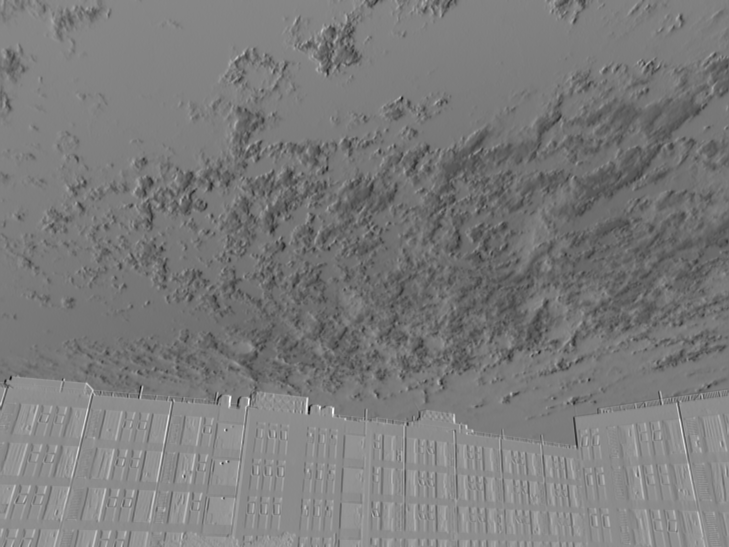
\includegraphics[width=\textwidth]{sky_sobel0.png}  %设置图片的输出大小倍数,这里是0.5倍大小输出
    \end{minipage}
    }
    \subfigure[y方向Sobel算子]{ %第二张子图
    \begin{minipage}{0.4\textwidth}
    \centering    %子图居中
    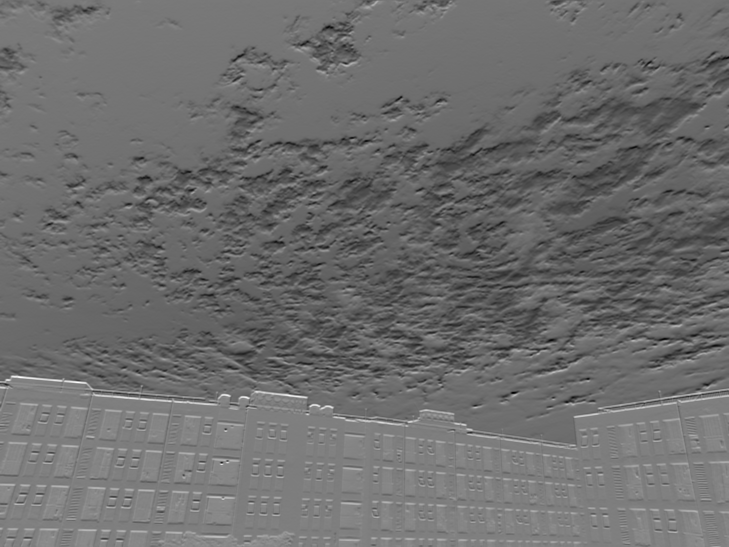
\includegraphics[width=\textwidth]{sky_sobel1.png}%以pic.jpg的0.5倍大小输出
    \end{minipage}
    }
    \\
        \subfigure[原始图像]{   %子图
        \begin{minipage}{0.4\textwidth}%大小总和超过textwidth则自动换行
        \centering    %子图居中
        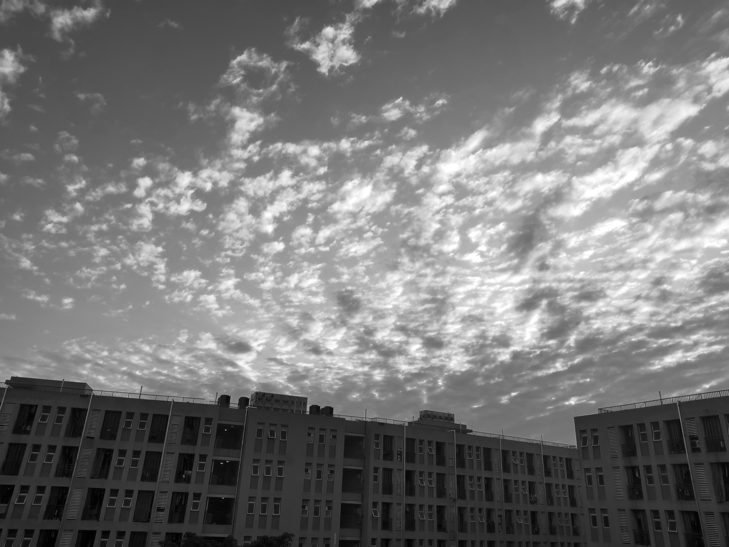
\includegraphics[width=\textwidth]{sky.png}  %设置图片的输出大小倍数,这里是0.5倍大小输出
        \end{minipage}
        }
    \caption{不同方向的sobel算子处理结果}    %大图名称
    \label{fig:1}    %图片引用标记
\end{figure}
如图可知,x方向和y方向的边缘被明显检测出来,为了得到整体响应,我们还需要对偏导算子进行不同范数的计算。使用不同范数的梯度响应图如图(\ref{sobelb})所示:

\begin{figure}[htbp]
    \centering  %居中
    \subfigure[1范数响应]{   %第一张子图
    \begin{minipage}{0.4\textwidth}%大小总和超过textwidth则自动换行
    \centering    %子图居中
    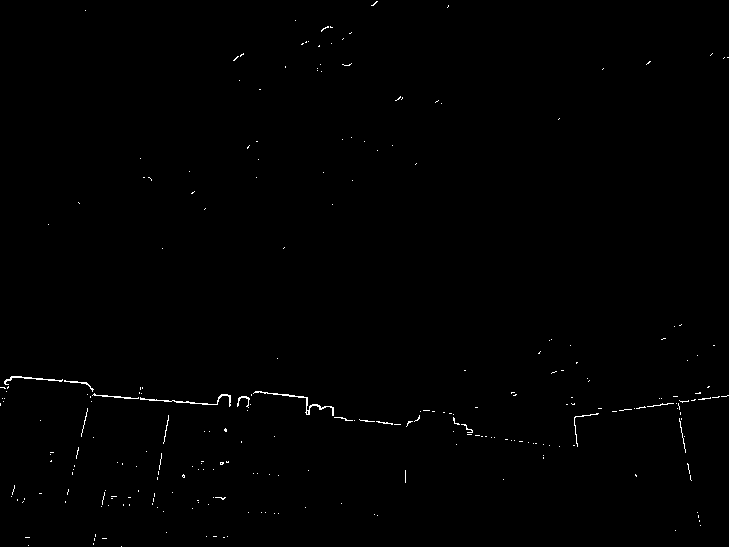
\includegraphics[width=\textwidth]{sky_sobel2b.png}  %设置图片的输出大小倍数,这里是0.5倍大小输出
    \end{minipage}
    }
    \subfigure[2范数响应]{ %第二张子图
    \begin{minipage}{0.4\textwidth}
    \centering    %子图居中
    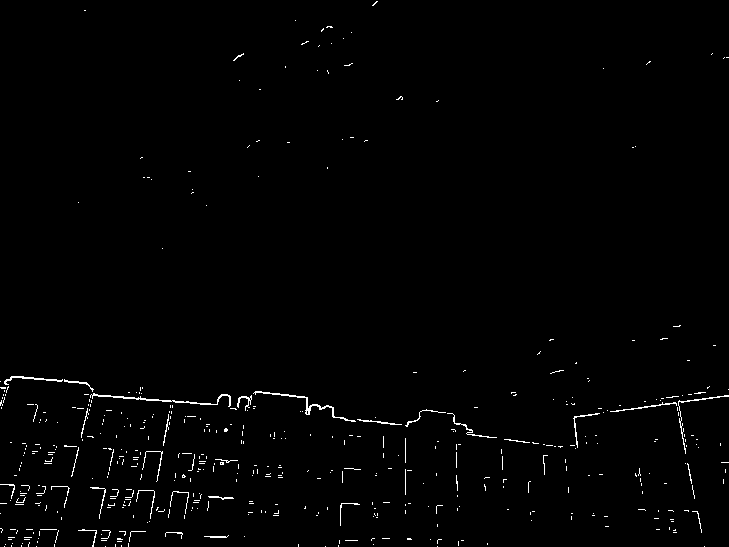
\includegraphics[width=\textwidth]{sky_sobel3b.png}%以pic.jpg的0.5倍大小输出
    \end{minipage}
    }
    \\
        \subfigure[无穷范数响应]{   %子图
        \begin{minipage}{0.4\textwidth}%大小总和超过textwidth则自动换行
        \centering    %子图居中
        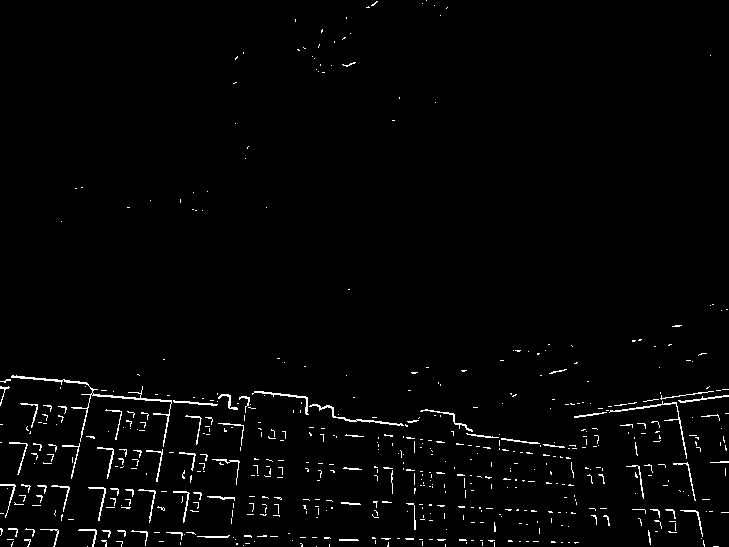
\includegraphics[width=\textwidth]{sky_sobel4b.png}  %设置图片的输出大小倍数,这里是0.5倍大小输出
        \end{minipage}
        }

    \caption{不同范数梯度图响应结果}    %大图名称
    \label{sobelb}    %图片引用标记
\end{figure}

可见二范数下图像梯度响应结果最好,这是因为该范数下各个方向的响应值都被计算到最终的响应中,而无穷范数只计算了两个方向响应的最大值,丢失了较小的方向响应结果。

\subsection{角点检测}
\subsubsection{二值图像中的角点检测结果}
在二值图像上使用SUSAN算子,得到图(\ref{susan_cuan})响应结果:
\begin {figure}[h]
\centering % 居中显示
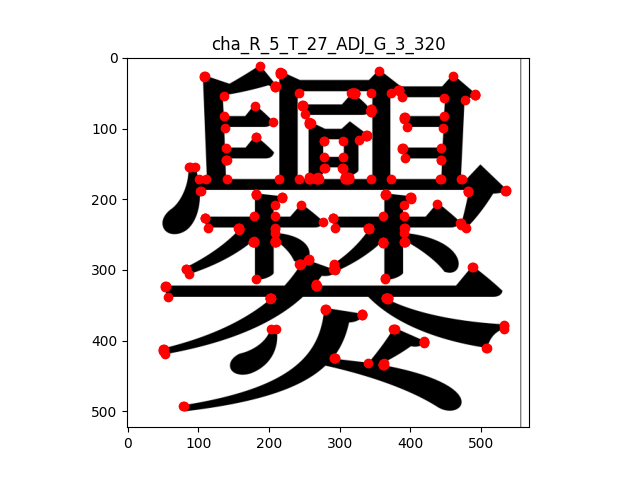
\includegraphics[width=0.4\textwidth]{susan_cuan.png}
\caption{SUSAN算子二值图像响应结果} % 标题
\label{susan_cuan}
\end {figure}

在调整了多次参数之后,设置半径为5,灰度阈值为27,最大面积为0.75倍模板大小获得了该结果。可见检测效果较好,几乎没有漏检错检的情况。

\subsubsection{真实图像上的角点检测结果}
在真实图像上使用SUSAN算子并没有获得一致的效果,首先添加了SUSAN的响应下限,认为核同值区域需要大于4倍半径才认为是角点。得到图(\ref{susan_obj_1})中的结果:
\begin{figure}[htbp]
    \centering  %居中
    \subfigure[原始SUSAN]{   %第一张子图
    \begin{minipage}{0.45\textwidth}%大小总和超过textwidth则自动换行
    \centering    %子图居中
    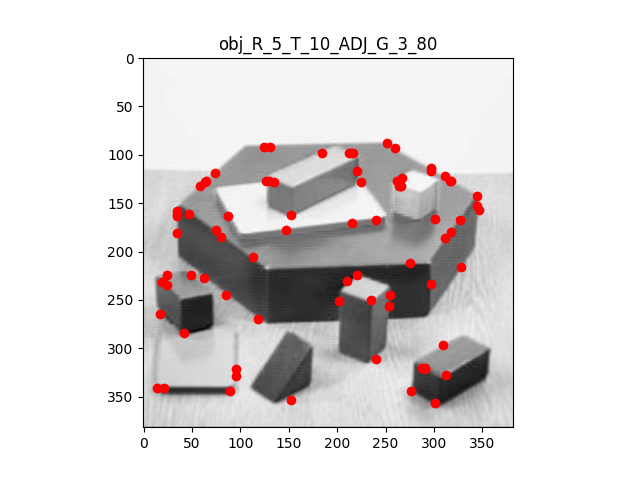
\includegraphics[width=\textwidth]{susan_obj_1_1.png}  %设置图片的输出大小倍数,这里是0.5倍大小输出
    \end{minipage}
    }
    \subfigure[指定半径下限为4r]{ %第二张子图
    \begin{minipage}{0.45\textwidth}
    \centering    %子图居中
    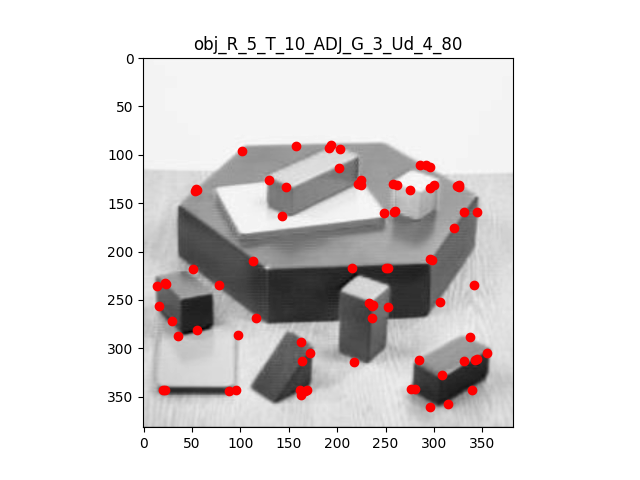
\includegraphics[width=\textwidth]{susan_obj_1_2.png}%以pic.jpg的0.5倍大小输出
    \end{minipage}
    }
    

    \caption{指定半径下限的SUSAN算子结果}    %大图名称
    \label{susan_obj_1}    %图片引用标记
\end{figure}
可见改进后的方法减少了部分位置错误识别的情况,但是带来了另一些部分角点的错误检测。为此,我又在添加响应下限的基础上改变半径为10,再次比对效果 (图\ref{susan_obj_2}):
\begin{figure}[htbp]
    \centering  %居中
    \subfigure[$r=5$]{   %第一张子图
    \begin{minipage}{0.4\textwidth}%大小总和超过textwidth则自动换行
    \centering    %子图居中
    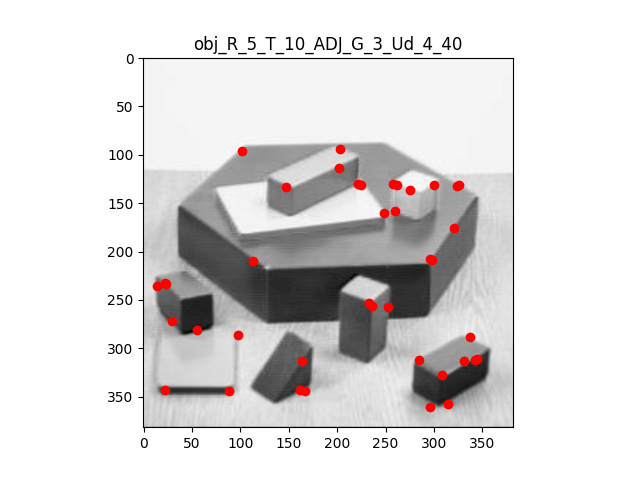
\includegraphics[width=\textwidth]{susan_obj_2_5.png}  %设置图片的输出大小倍数,这里是0.5倍大小输出
    \end{minipage}
    }
    \subfigure[$r=10$]{ %第二张子图
    \begin{minipage}{0.4\textwidth}
    \centering    %子图居中
    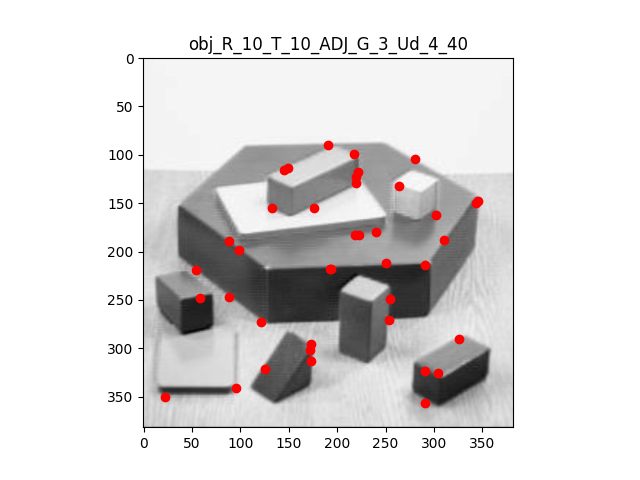
\includegraphics[width=\textwidth]{susan_obj_2_10.png}%以pic.jpg的0.5倍大小输出
    \end{minipage}
    }
    

    \caption{不同半径范围下的SUSAN算子检测效果}    %大图名称
    \label{susan_obj_2}    %图片引用标记
\end{figure}

SUSAN算子半径增加后反而带来更多误分类,说明对于边缘模糊的现实图像,SUSAN算子表现并不好。我将在后面分析二值图像和现实图像的差异,以分析为何SUSAN算子表现不好的原因。

\subsubsection{不同图片的对比}
SUSAN算子在二值图像和真实图像的检测效果不同,本质上是因为边缘模糊或者是形状复杂,导致错误识别角点。观察图(\ref{su_c}),可以直观对比二者差异。
\begin{figure}[htbp]
    \centering  %居中
    \subfigure[二值角点]{   %第一张子图
    \begin{minipage}{0.3\textwidth}%大小总和超过textwidth则自动换行
    \centering    %子图居中
    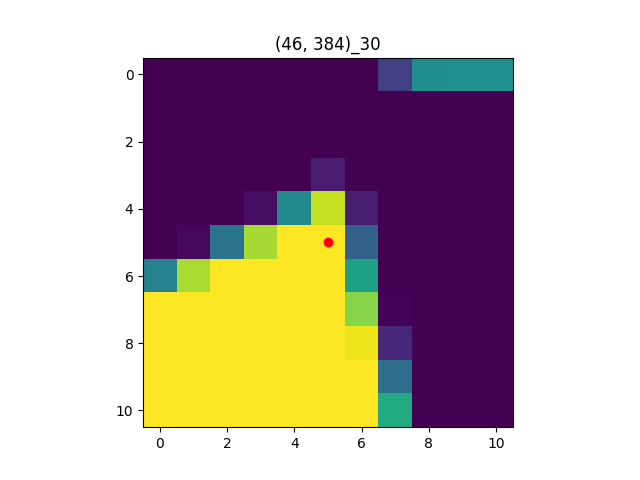
\includegraphics[width=\textwidth]{su_c_b.png}  %设置图片的输出大小倍数,这里是0.5倍大小输出
    \end{minipage}
    }
    \subfigure[错误检测边缘]{ %第二张子图
    \begin{minipage}{0.3\textwidth}
    \centering    %子图居中
    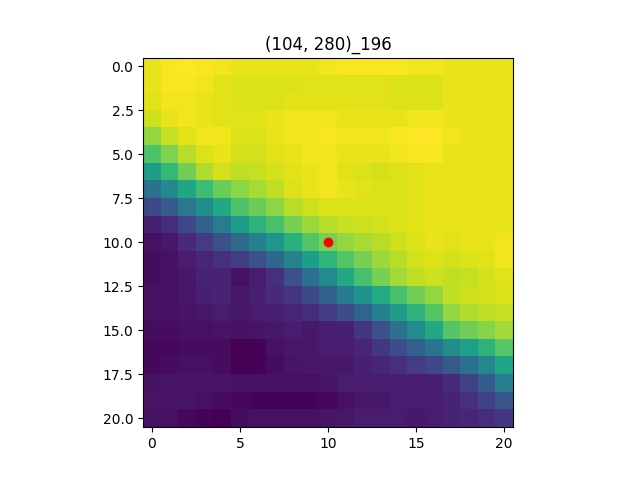
\includegraphics[width=\textwidth]{su_c_er.png}%以pic.jpg的0.5倍大小输出
    \end{minipage}
    }
        \subfigure[错误检测复杂区域]{   %子图
        \begin{minipage}{0.3\textwidth}%大小总和超过textwidth则自动换行
        \centering    %子图居中
        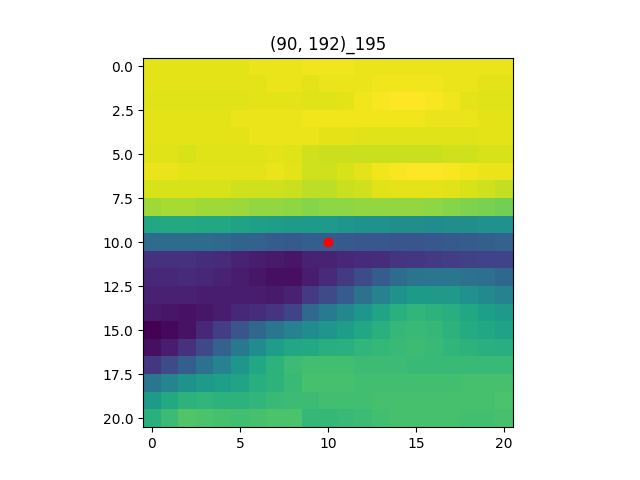
\includegraphics[width=\textwidth]{su_c_di.png}  %设置图片的输出大小倍数,这里是0.5倍大小输出
        \end{minipage}
        }

    \caption{角点检测局部细节}    %大图名称
    \label{su_c}    %图片引用标记
\end{figure}

在真实图像的检测中,模糊的边缘对角点检测的效果影响很大,而如果设置较小的阈值,又会导致噪声不敏感以及遗漏角点的现象。因此,我们需要探寻新的方法进行真实图像上的角点检测。

\subsection{DoG算法}
使用DoG算法对原始图像再次检测角点,得到以下结果:图(\ref{DoG})
\begin{figure}[htbp]
    \centering  %居中
    \subfigure[DoG处理结果]{   %第一张子图
    \begin{minipage}{0.4\textwidth}%大小总和超过textwidth则自动换行
    \centering    %子图居中
    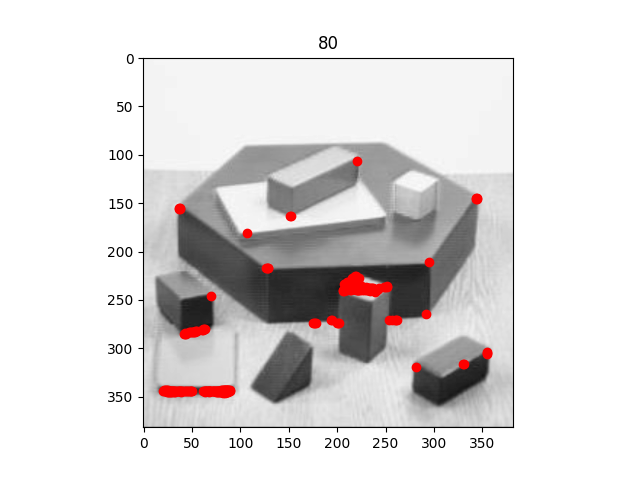
\includegraphics[width=\textwidth]{80.png}  %设置图片的输出大小倍数,这里是0.5倍大小输出
    \end{minipage}
    }
    \subfigure[SUSAN算子处理结果]{ %第二张子图
    \begin{minipage}{0.4\textwidth}
    \centering    %子图居中
    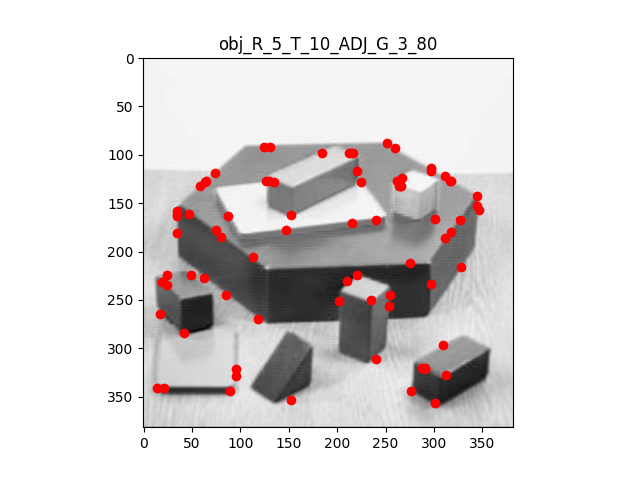
\includegraphics[width=\textwidth]{susan_obj_1_1.png}%以pic.jpg的0.5倍大小输出
    \end{minipage}
    }
    
    \caption{DoG与SUSAN处理结果对比}    %大图名称
    \label{DoG}    %图片引用标记
\end{figure}

DoG算法几乎没有出现边缘点的误分类,但是出现了图形内部错误识别为角点的问题。这可能是高$\sigma$数值下的错误响应,可以添加最小响应阈值消除。
\section{总结及心得体会:}

在本次实验中,我基本掌握和复现了常用的图像基元检测算法。并且通过前后图像对比,直观认识了不同处理方法的效果以及特点。在这一基础上,我在角点检测这一方面展开研究,并且复现了DoG代码。

在本次图像基本操作的实验中,我加深了对一些常见图像处理方法的认知,锻炼了自己的编码能力。在基本要求的基础上,我还寻找了直方图均衡化的创新算法:DoG,对课内知识做了补充。在这一过程中,我锻炼了自己信息检索的能力,以及阅读相关文献资料的能力。

\section{对本实验过程及方法、手段的改进建议:}
\begin{enumerate}
  \item \textbf{边缘检测:} 可以尝试多种边缘检测的模板,在不同图像上实验模板效果,对比差异。
  \item \textbf{角点检测:} 尝试查阅相关资料,实现改进的SUSAN算子方法。
  \item \textbf{DoG角点检测:} 添加最小响应阈值,以消除区域内部的误检测。 
\end{enumerate}

\vspace{4cm}
\begin{flushright}
\begin{tabular}{lc}
\sihao{\hei{报告评分:}}& \sihao{\vspace{10pt}}\\
\sihao{\hei{指导教师签字:}}& \sihao{\vspace{10pt}}\\
\end{tabular}
\end{flushright}
\newpage

\bibliography{ref}
\bibliographystyle{IEEEtran}

% {\noindent\hei \sihao 代码实现}
\end{document}
